\section{Inleiding}

De term \emph{computernetwerk} bestaat uit twee woorden: ``computer'' en ``netwerk.''
Wikipedia definiëert een \emph{computer} als een ``apparaat waarmee gegevens volgens formele procedures verwerkt kunnen worden.''
Dat is echter een nogal vage definitie.
Gelukkig hebben we allemaal wel een goed idee van wat een computer is: een laptop of desktop computer.
Maar ook servers, netwerkprinters, tablets en gsm-toestellen zijn volwaardige computers.
Meer nog, tegenwoordig zit er zelfs een computer in je auto of het mengpaneel van een muziekinstallatie!

Een \emph{netwerk} is, volgens Wikipedia, een ``systeem voor communicatie tussen twee of meer computers.''
Hier denken we dan misschien meteen aan het wireless netwerk of de ``internetkabel'' op kantoor of bij je thuis;
maar je kan ook netwerken maken met infrarood (IrDA), bluetooth of 5G.
Glasvezel, ADSL en coax zijn ook voorbeelden van computernetwerken.



\subsection{Netwerkprotocollen}

Een protocol is, om weeral Wikipedia te citeren, een ``gedragsovereenkomst, meestal in de vorm van een aantal uit te voeren stappen.''
Het vormt dus een set regels waar twee computers zich aan willen houden, als ze met elkaar willen communiceren.
We kunnen dit vergelijken met enkele gedragsregels uit het dagelijks leven.
Als je een nieuw persoon ontmoet, schud je elkaar de hand en stel je jezelf kort voor.%
  \footnote{Covid-19 heeft er voor gezorgd dat er een ander protocol gebruikt wordt in deze (en vele andere) situatie.}
In de klas zwijgt iedereen zodat de docent zijn uitleg kan doen.
Als je een vraag wil stellen, steek je de hand omhoog en wacht je tot de docent stopt met praten en jou aanduidt zodat jij aan het woord mag.
Als je de koning mag ontmoeten, moet je een heel nieuw protocol leren voor de interactie.

Computernetwerken gebruiken ook verschillende protocollen.
Enkele protocollen die we in deze cursus (kort) zullen behandelen, zijn
IPv4 en IPv6, TCP en UDP, Ethernet en ARP.
Enkele protocollen die niet meer gebruikt worden in computernetwerken, zijn IPX, SPX en AppleTalk.



\subsection{Evolutie in netwerken}

De eerste \emph{mainframes} stammen uit de jaren 50.
De gegevens werden oorspronkelijk ingevoerd met gegevensdragers als ponskaarten, ponsbanden en magneetbanden.
In de jaren 70 werden op enige schaal terminals aan mainframes aangesloten, aanvankelijk schrijfmachineterminals en later ook beeldschermen.

In 1971 werd ALOHAnet in gebruik genomen in Hawaï.
Dit was het eerste draadloos computernetwerk.
In 1973--74 werd Ethernet ontwikkeld op basis van dit draadloos netwerk.
Ethernet gebruikte eerst thicknet (1982), daarna thinnet (1983), en vervolgens twisted pair (1984).
Concurrerende protocollen waren Token Ring (1984) en FDDI (1987).
Begin jaren 90 kwamen de Ethernetswitches en verdrong Ethernet vrij snel alle andere protocollen.



\subsection{Netwerktopologieën}

De meet eenvoudige topologie is een point-to-pointverbinding tussen twee computers door beide computers rechtstreeks met elkaar te verbindinen met een kabel.
Deze topologie schaalt echter niet goed.
Voorbeelden van kabels zijn een seriële kabel, een coax\-kabel of een UTP-kabel.

Thick- en thinnet gebruikten beide een fysieke busstructuur waarbij alle computers op één lange kabel geprikt werden.
Beide standaarden gebruikten coax (echter van een andere dikte, vandaar de namen) maar beide gebruikten een andere manier om de computers met het netwerk te verbinden.
Thicknet gebruikte ``vampire taps'' terwijl thinnet BNC-koppelstukken gebruikte.%
   \footnote{Er was ook een N-connector beschikbaar voor Thicknet maar deze werd blijkbaar amper gebruikt (\href{http://www.mattmillman.com/projects/10base5/}{bron}).}

Hoewel Token Ring een fysieke stertopologie had -- met een centrale media access unit (MAU) -- vormden de kabels een ringtopologie.
Hubs en switches vormen ook een fysieke stertopologie.
Een hub werkt functioneel zoals thinnet en vormt aldus een logische busstructuur terwijl een switch als een reeks logische point-to-pointverbindingen werkt.

Een \emph{full mesh} netwerk is een netwerk waarbij elk toestel met elk ander toestel verbonden is door middel van point-to-pointverbindingen.
Een \emph{partial mesh} netwerk is een netwerk waarbij een deel van de directe verbindingen van een full mesh ontbreken.

\subsection{Het OSI-model en het TCP/IP-model}

Het OSI-model is een conceptueel model voor netwerkcommunicatie.
Het werd als theoretisch model ontwikkeld met de bedoeling dat de praktijk zich aan dit model aan zou passen.
Het TCP/IP-model is een alternatief protocol dat gebaseerd is op de protocollen die al in de praktijk gebruikt werden.

\begin{table}[htp]
   \centering
   \begin{tabular}{rll}
   \toprule
     & \textit{OSI-model} & \textit{TCP/IP-model} \\
   \midrule
   7 & application & \multirow{3}{*}{\textcolor{spot1}{application}} \\
   6 & presentation & \\
   5 & session & \\[1ex]
   4 & \textcolor{spot1}{transport} & transport \\[1ex]
   3 & \textcolor{spot1}{network} & internet \\[1ex]
   2 & \textcolor{spot1}{data link} & \multirow{2}{*}{link} \\
   1 & \textcolor{spot1}{physical} & \\
   \bottomrule
   \end{tabular}
   \caption{De zeven lagen van het OSI-model en de vier lagen van het TCP/IP-model.
   De vijf lagen van het hybride model zijn in het rood weergegeven.}
   \label{tab:osi-model}
\end{table}

Deze modellen hebben weinig praktisch nut maar kunnen wel helpen met het gestructureerd opsporen en oplossen van netwerkproblemen.
Afhankelijk van het probleem kan je ofwel op laag~7 (de applicatie) beginnen met troubleshooten, ofwel op laag~1 (bekabeling), ofwel in het midden op laag~3 (\cmd{ping} en \cmd{traceroute}).
Onderstaand vind je voor de vijf lagen van het hybride model enkele zaken die onderzocht kunnen worden.

\begin{description}
\item[application]
   Controleer de configuratie van de applicatie zelf.
   Dit is voor de applicatie- of systeembeheerders en niet meer voor de netwerkbeheerder.
\item[transport]
   Controleer firewallconfiguraties en of de service (applicatie) wel gestart is op de server.
   Je kan met behulp van \cmd{telnet} testen of de applicatie bereikbaar is.
\item[network]
   Verifiëer met behulp van \cmd{ping} en \cmd{traceroute} of de twee computers elkaar kunnen bereiken.
   De output van \cmd{traceroute} geeft een indicatie hoe de pakketjes doorheen het netwerk gaan.
   Dit kan je best in beide richtingen controleren aangezien \emph{asymetrisch} netwerkverkeer mogelijk is en mogelijk voor problemen kan zorgen.
\item[data link]
   Op het lokale netwerk moet je zaken zoals Spanning-tree protocol (STP) en VLAN-configuraties nakijken.
   Zaken zoals DHCP snooping, dynamic ARP inspection (DAI) en port security kan je hier ook nakijken.
\item[physical]
  Controleer bekabeling, connectors, interface errors en, in het geval van wifi, mogelijke storingsbronnen.
\end{description}

De verschillende lagen vinden we ook terug als we de verschillende stappen doorlopen die computers doorlopen om met elkaar te communiceren.



\subsection{Communicatie tussen computers}

Nemen we als voorbeeld een computer, de \emph{client}, die een webpagina wil ophalen van een andere computer, de \emph{server} (\vref{fig:client-server}).
Het protocol dat hier voor gebruikt wordt, heet hypertext transfer protocol (HTTP).
De client verstuurt een HTTP \emph{request} en de server antwoordt met een HTTP \emph{response}.

De request bevat de volgende data.
\begin{verbatim}
GET /index.html HTTP/1.1
Host: www.example.com
\end{verbatim}

\begin{figure}
   \centering
   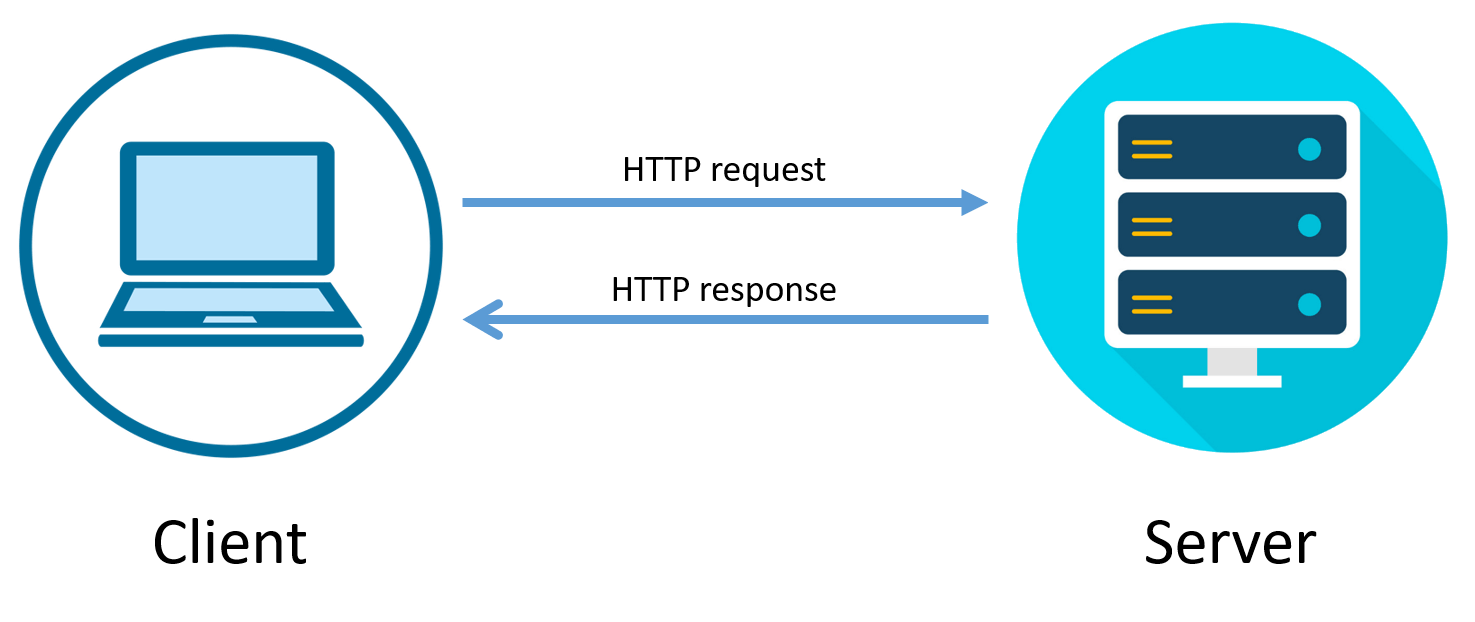
\includegraphics[width=.65\textwidth]{images/http-request.png}
   \caption{Een client vraagt een webpagina op bij eeen webserver en gebruikt voor deze communicatie HTTP}
   \label{fig:client-server}
\end{figure}

Het antwoord van de server bevat enerzijds de HTTP-data die het protocol vereist, en anderzijds de gevraagd webpagina.
In dit geval bevat de gevraagde pagina HTML-code.
\begin{verbatim}
HTTP/1.1 200 OK
Content-Type: text/html; charset=UTF-8
Content-Length: 155
Server: Apache/1.3.3.7 (Unix) (Red-Hat/Linux)

<html>
  <head><title>An Example Page</title></head>
  <body><p>Hello World!</p></body>
</html>
\end{verbatim}

Dit ogenschijnlijk eenvoudig voorbeeld roept toch meerdere vragen op.
\begin{enumerate}
\item Hoe kunnen we de server bereiken?
\item Voor welke applicatie is de data bestemd?
\item Hoe versturen we heel veel data?
\item Wat doen we als er iets mis gaat?
\end{enumerate}






\begin{frame}{Hoe de server bereiken?}
\begin{itemize}
\item<1-> DNS-naam
    \begin{itemize}
    \item Adresbalk: \url{http://www.example.com/}
    \item Hostheader: www.example.com
    \end{itemize}
\item<2-> IP-adres
\end{itemize}
\end{frame}



\begin{frame}{Voor welke applicatie is de data bestemd?}
\begin{itemize}[<+->]
\item Elke serverapplicatie luistert op een bepaalde ``poort''
\item Computerstandaarden bepalen poortnummers
\item De client gebruikt een willekeurige poort
\end{itemize}
\end{frame}



\begin{frame}{Hoe versturen we heel veel data?}
\begin{itemize}[<+->]
\item Fragmentatie: opsplitsen in kleine pakketjes
\item Volgorde van de fragmenten
\end{itemize}
\end{frame}



\begin{frame}{Wat als er dingen mis gaan?}
\begin{itemize}[<+->]
\item Pakketjes kunnen verloren gaan
\item Er kunnen fouten optreden in de data
\item Pakketjes kunnen in de verkeerde volgorde aankomen
\end{itemize}
\end{frame}



\subsection{Verschillende lagen en modellen}

\begin{frame}{Verschillende lagen}
\begin{itemize}[<+->]
\item Structuur brengt orde
\item Vereenvoudigt troubleshooten
\item Maakt protocollen vervangbaar
    \begin{example}
    bv IPv4 wordt IPv6
    \end{example}
\end{itemize}
\end{frame}

\mode<article>{
In deze cursus zoeken we het antwoord op deze vragen en ontdekken we hoe computernetwerk opgebouwd zijn en hoe je kan communiceren tussen verschillende netwerken.

De industrie heeft een aantal verschillende maar gelijkaardige modellen in het leven geroepen om stuctuur te brengen in de verschillende protocollen.
De theorie en geschiedenis zijn niet belangrijk, maar een basiskennis van deze protocollen helpt wel om alles te plaatsen en om netwerkproblemen op te sporen en op te lossen.
}





\begin{frame}{Communicatie gebeurt tussen lagen onderling}
\begin{center}
\includegraphics<presentation>[width=\textwidth]{images/tcpip_5_layer_overview.png}
\includegraphics<article>[width=.65\textwidth]{images/tcpip_5_layer_overview.png}
\end{center}
Bron: \url{https://microchipdeveloper.com/}
\end{frame}



\begin{frame}{Elke laag voegt een header toe}
\begin{center}
\includegraphics<presentation>[width=\textwidth]{images/transmit_data.jpg}
\includegraphics<article>[width=.65\textwidth]{images/transmit_data.jpg}
\end{center}
Bron: \url{https://microchipdeveloper.com/}
\end{frame}



\begin{frame}{Voorbeeld}
\begin{itemize}
\item Applicatielaag: HTTP client request
\item Transportlaag: TCP-poort 80 voor HTTP
\item Netwerklaag: IP-adres van client en server
\item Datalinklaag: MAC-adressen
\item Fysieke laag: stroom of licht op de kabel
\end{itemize}
\end{frame}



\subsection{Netwerktopologieën}

\begin{frame}{Netwerktopologieën}
\begin{itemize}[<+->]
\item point-to-point
\item daisy chain (linear or ring)
\item bus
\item ster
\item mesh
\end{itemize}
\end{frame}

\mode<article>{
Deze verschillende topologieën komen we tijdens de cursus tegen dus benoemen we deze eerst kort. 
}


\subsection{Evolutie in netwerken}

